% Options for packages loaded elsewhere
\PassOptionsToPackage{unicode}{hyperref}
\PassOptionsToPackage{hyphens}{url}
%
\documentclass[
  ignorenonframetext,
]{beamer}
\usepackage{pgfpages}
\setbeamertemplate{caption}[numbered]
\setbeamertemplate{caption label separator}{: }
\setbeamercolor{caption name}{fg=normal text.fg}
\beamertemplatenavigationsymbolsempty
% Prevent slide breaks in the middle of a paragraph
\widowpenalties 1 10000
\raggedbottom
\setbeamertemplate{part page}{
  \centering
  \begin{beamercolorbox}[sep=16pt,center]{part title}
    \usebeamerfont{part title}\insertpart\par
  \end{beamercolorbox}
}
\setbeamertemplate{section page}{
  \centering
  \begin{beamercolorbox}[sep=12pt,center]{part title}
    \usebeamerfont{section title}\insertsection\par
  \end{beamercolorbox}
}
\setbeamertemplate{subsection page}{
  \centering
  \begin{beamercolorbox}[sep=8pt,center]{part title}
    \usebeamerfont{subsection title}\insertsubsection\par
  \end{beamercolorbox}
}
\AtBeginPart{
  \frame{\partpage}
}
\AtBeginSection{
  \ifbibliography
  \else
    \frame{\sectionpage}
  \fi
}
\AtBeginSubsection{
  \frame{\subsectionpage}
}

\usepackage{amsmath,amssymb}
\usepackage{lmodern}
\usepackage{iftex}
\ifPDFTeX
  \usepackage[T1]{fontenc}
  \usepackage[utf8]{inputenc}
  \usepackage{textcomp} % provide euro and other symbols
\else % if luatex or xetex
  \usepackage{unicode-math}
  \defaultfontfeatures{Scale=MatchLowercase}
  \defaultfontfeatures[\rmfamily]{Ligatures=TeX,Scale=1}
\fi
\usetheme[]{simplecustom.scss}
% Use upquote if available, for straight quotes in verbatim environments
\IfFileExists{upquote.sty}{\usepackage{upquote}}{}
\IfFileExists{microtype.sty}{% use microtype if available
  \usepackage[]{microtype}
  \UseMicrotypeSet[protrusion]{basicmath} % disable protrusion for tt fonts
}{}
\makeatletter
\@ifundefined{KOMAClassName}{% if non-KOMA class
  \IfFileExists{parskip.sty}{%
    \usepackage{parskip}
  }{% else
    \setlength{\parindent}{0pt}
    \setlength{\parskip}{6pt plus 2pt minus 1pt}}
}{% if KOMA class
  \KOMAoptions{parskip=half}}
\makeatother
\usepackage{xcolor}
\newif\ifbibliography
\setlength{\emergencystretch}{3em} % prevent overfull lines
\setcounter{secnumdepth}{-\maxdimen} % remove section numbering

\usepackage{color}
\usepackage{fancyvrb}
\newcommand{\VerbBar}{|}
\newcommand{\VERB}{\Verb[commandchars=\\\{\}]}
\DefineVerbatimEnvironment{Highlighting}{Verbatim}{commandchars=\\\{\}}
% Add ',fontsize=\small' for more characters per line
\usepackage{framed}
\definecolor{shadecolor}{RGB}{241,243,245}
\newenvironment{Shaded}{\begin{snugshade}}{\end{snugshade}}
\newcommand{\AlertTok}[1]{\textcolor[rgb]{0.68,0.00,0.00}{#1}}
\newcommand{\AnnotationTok}[1]{\textcolor[rgb]{0.37,0.37,0.37}{#1}}
\newcommand{\AttributeTok}[1]{\textcolor[rgb]{0.40,0.45,0.13}{#1}}
\newcommand{\BaseNTok}[1]{\textcolor[rgb]{0.68,0.00,0.00}{#1}}
\newcommand{\BuiltInTok}[1]{\textcolor[rgb]{0.00,0.23,0.31}{#1}}
\newcommand{\CharTok}[1]{\textcolor[rgb]{0.13,0.47,0.30}{#1}}
\newcommand{\CommentTok}[1]{\textcolor[rgb]{0.37,0.37,0.37}{#1}}
\newcommand{\CommentVarTok}[1]{\textcolor[rgb]{0.37,0.37,0.37}{\textit{#1}}}
\newcommand{\ConstantTok}[1]{\textcolor[rgb]{0.56,0.35,0.01}{#1}}
\newcommand{\ControlFlowTok}[1]{\textcolor[rgb]{0.00,0.23,0.31}{#1}}
\newcommand{\DataTypeTok}[1]{\textcolor[rgb]{0.68,0.00,0.00}{#1}}
\newcommand{\DecValTok}[1]{\textcolor[rgb]{0.68,0.00,0.00}{#1}}
\newcommand{\DocumentationTok}[1]{\textcolor[rgb]{0.37,0.37,0.37}{\textit{#1}}}
\newcommand{\ErrorTok}[1]{\textcolor[rgb]{0.68,0.00,0.00}{#1}}
\newcommand{\ExtensionTok}[1]{\textcolor[rgb]{0.00,0.23,0.31}{#1}}
\newcommand{\FloatTok}[1]{\textcolor[rgb]{0.68,0.00,0.00}{#1}}
\newcommand{\FunctionTok}[1]{\textcolor[rgb]{0.28,0.35,0.67}{#1}}
\newcommand{\ImportTok}[1]{\textcolor[rgb]{0.00,0.46,0.62}{#1}}
\newcommand{\InformationTok}[1]{\textcolor[rgb]{0.37,0.37,0.37}{#1}}
\newcommand{\KeywordTok}[1]{\textcolor[rgb]{0.00,0.23,0.31}{#1}}
\newcommand{\NormalTok}[1]{\textcolor[rgb]{0.00,0.23,0.31}{#1}}
\newcommand{\OperatorTok}[1]{\textcolor[rgb]{0.37,0.37,0.37}{#1}}
\newcommand{\OtherTok}[1]{\textcolor[rgb]{0.00,0.23,0.31}{#1}}
\newcommand{\PreprocessorTok}[1]{\textcolor[rgb]{0.68,0.00,0.00}{#1}}
\newcommand{\RegionMarkerTok}[1]{\textcolor[rgb]{0.00,0.23,0.31}{#1}}
\newcommand{\SpecialCharTok}[1]{\textcolor[rgb]{0.37,0.37,0.37}{#1}}
\newcommand{\SpecialStringTok}[1]{\textcolor[rgb]{0.13,0.47,0.30}{#1}}
\newcommand{\StringTok}[1]{\textcolor[rgb]{0.13,0.47,0.30}{#1}}
\newcommand{\VariableTok}[1]{\textcolor[rgb]{0.07,0.07,0.07}{#1}}
\newcommand{\VerbatimStringTok}[1]{\textcolor[rgb]{0.13,0.47,0.30}{#1}}
\newcommand{\WarningTok}[1]{\textcolor[rgb]{0.37,0.37,0.37}{\textit{#1}}}

\providecommand{\tightlist}{%
  \setlength{\itemsep}{0pt}\setlength{\parskip}{0pt}}\usepackage{longtable,booktabs,array}
\usepackage{calc} % for calculating minipage widths
\usepackage{caption}
% Make caption package work with longtable
\makeatletter
\def\fnum@table{\tablename~\thetable}
\makeatother
\usepackage{graphicx}
\makeatletter
\def\maxwidth{\ifdim\Gin@nat@width>\linewidth\linewidth\else\Gin@nat@width\fi}
\def\maxheight{\ifdim\Gin@nat@height>\textheight\textheight\else\Gin@nat@height\fi}
\makeatother
% Scale images if necessary, so that they will not overflow the page
% margins by default, and it is still possible to overwrite the defaults
% using explicit options in \includegraphics[width, height, ...]{}
\setkeys{Gin}{width=\maxwidth,height=\maxheight,keepaspectratio}
% Set default figure placement to htbp
\makeatletter
\def\fps@figure{htbp}
\makeatother

\makeatletter
\makeatother
\makeatletter
\makeatother
\makeatletter
\@ifpackageloaded{caption}{}{\usepackage{caption}}
\AtBeginDocument{%
\ifdefined\contentsname
  \renewcommand*\contentsname{Table of contents}
\else
  \newcommand\contentsname{Table of contents}
\fi
\ifdefined\listfigurename
  \renewcommand*\listfigurename{List of Figures}
\else
  \newcommand\listfigurename{List of Figures}
\fi
\ifdefined\listtablename
  \renewcommand*\listtablename{List of Tables}
\else
  \newcommand\listtablename{List of Tables}
\fi
\ifdefined\figurename
  \renewcommand*\figurename{Figure}
\else
  \newcommand\figurename{Figure}
\fi
\ifdefined\tablename
  \renewcommand*\tablename{Table}
\else
  \newcommand\tablename{Table}
\fi
}
\@ifpackageloaded{float}{}{\usepackage{float}}
\floatstyle{ruled}
\@ifundefined{c@chapter}{\newfloat{codelisting}{h}{lop}}{\newfloat{codelisting}{h}{lop}[chapter]}
\floatname{codelisting}{Listing}
\newcommand*\listoflistings{\listof{codelisting}{List of Listings}}
\makeatother
\makeatletter
\@ifpackageloaded{caption}{}{\usepackage{caption}}
\@ifpackageloaded{subcaption}{}{\usepackage{subcaption}}
\makeatother
\makeatletter
\@ifpackageloaded{tcolorbox}{}{\usepackage[many]{tcolorbox}}
\makeatother
\makeatletter
\@ifundefined{shadecolor}{\definecolor{shadecolor}{rgb}{.97, .97, .97}}
\makeatother
\makeatletter
\makeatother
\ifLuaTeX
  \usepackage{selnolig}  % disable illegal ligatures
\fi
\IfFileExists{bookmark.sty}{\usepackage{bookmark}}{\usepackage{hyperref}}
\IfFileExists{xurl.sty}{\usepackage{xurl}}{} % add URL line breaks if available
\urlstyle{same} % disable monospaced font for URLs
\hypersetup{
  pdftitle={Workflow},
  pdfauthor={Data Analytics Unit},
  hidelinks,
  pdfcreator={LaTeX via pandoc}}

\title{Workflow}
\author{Data Analytics Unit}
\date{}

\begin{document}
\frame{\titlepage}
\ifdefined\Shaded\renewenvironment{Shaded}{\begin{tcolorbox}[frame hidden, boxrule=0pt, enhanced, sharp corners, borderline west={3pt}{0pt}{shadecolor}, breakable, interior hidden]}{\end{tcolorbox}}\fi

\hypertarget{workflow-definition}{%
\section{Workflow Definition}\label{workflow-definition}}

\begin{frame}{Workflow Definition and Features}
\protect\hypertarget{workflow-definition-and-features}{}
\begin{itemize}
\item
  A workflow is a system for managing repetitive processes and tasks
  which occur in a particular order.

  \begin{itemize}
  \tightlist
  \item
    Output recognition
  \item
    Process understanding
  \item
    Tasks that compose the process
  \item
    Tasks simplification
  \end{itemize}
\item
  Why we need so much structure?
  \href{https://hrdag.org/2016/06/14/the-task-is-a-quantum-of-workflow/}{\textbf{Human
  Rights Data Analysis Group}}

  \begin{itemize}
  \tightlist
  \item
    We can record and improve our process
  \item
    We can learn from the past
  \item
    We can read each other work
  \item
    We can test whether what we've done is correct
  \end{itemize}
\end{itemize}
\end{frame}

\begin{frame}{Workflow tools: git and SharePoint}
\protect\hypertarget{workflow-tools-git-and-sharepoint}{}
\begin{itemize}
\item
  Git is a free and open source software that allows users to set up a
  version control system designed to handle projects. For more
  information:
  \href{https://kinsta.com/knowledgebase/what-is-github/}{\textbf{What
  is github?}}

  \begin{itemize}
  \tightlist
  \item
    GitHub is a website and cloud-based service that helps developers
    store and manage their code, as well as track and control changes to
    their code.
  \item
    Using the Git features allow us to simultaneously work on the same
    project and even in the same code without worrying about interfering
    with other members of the team.
  \end{itemize}
\item
  Git is only used as a code repository. We don't share any data and
  output here.
\item
  Git can be linked and integrated with SharePoint. As a result, our
  workflow is contingent upon the manner in which our team chooses to
  structure our folders.
\end{itemize}
\end{frame}

\begin{frame}{Workflow tools: some examples}
\protect\hypertarget{workflow-tools-some-examples}{}
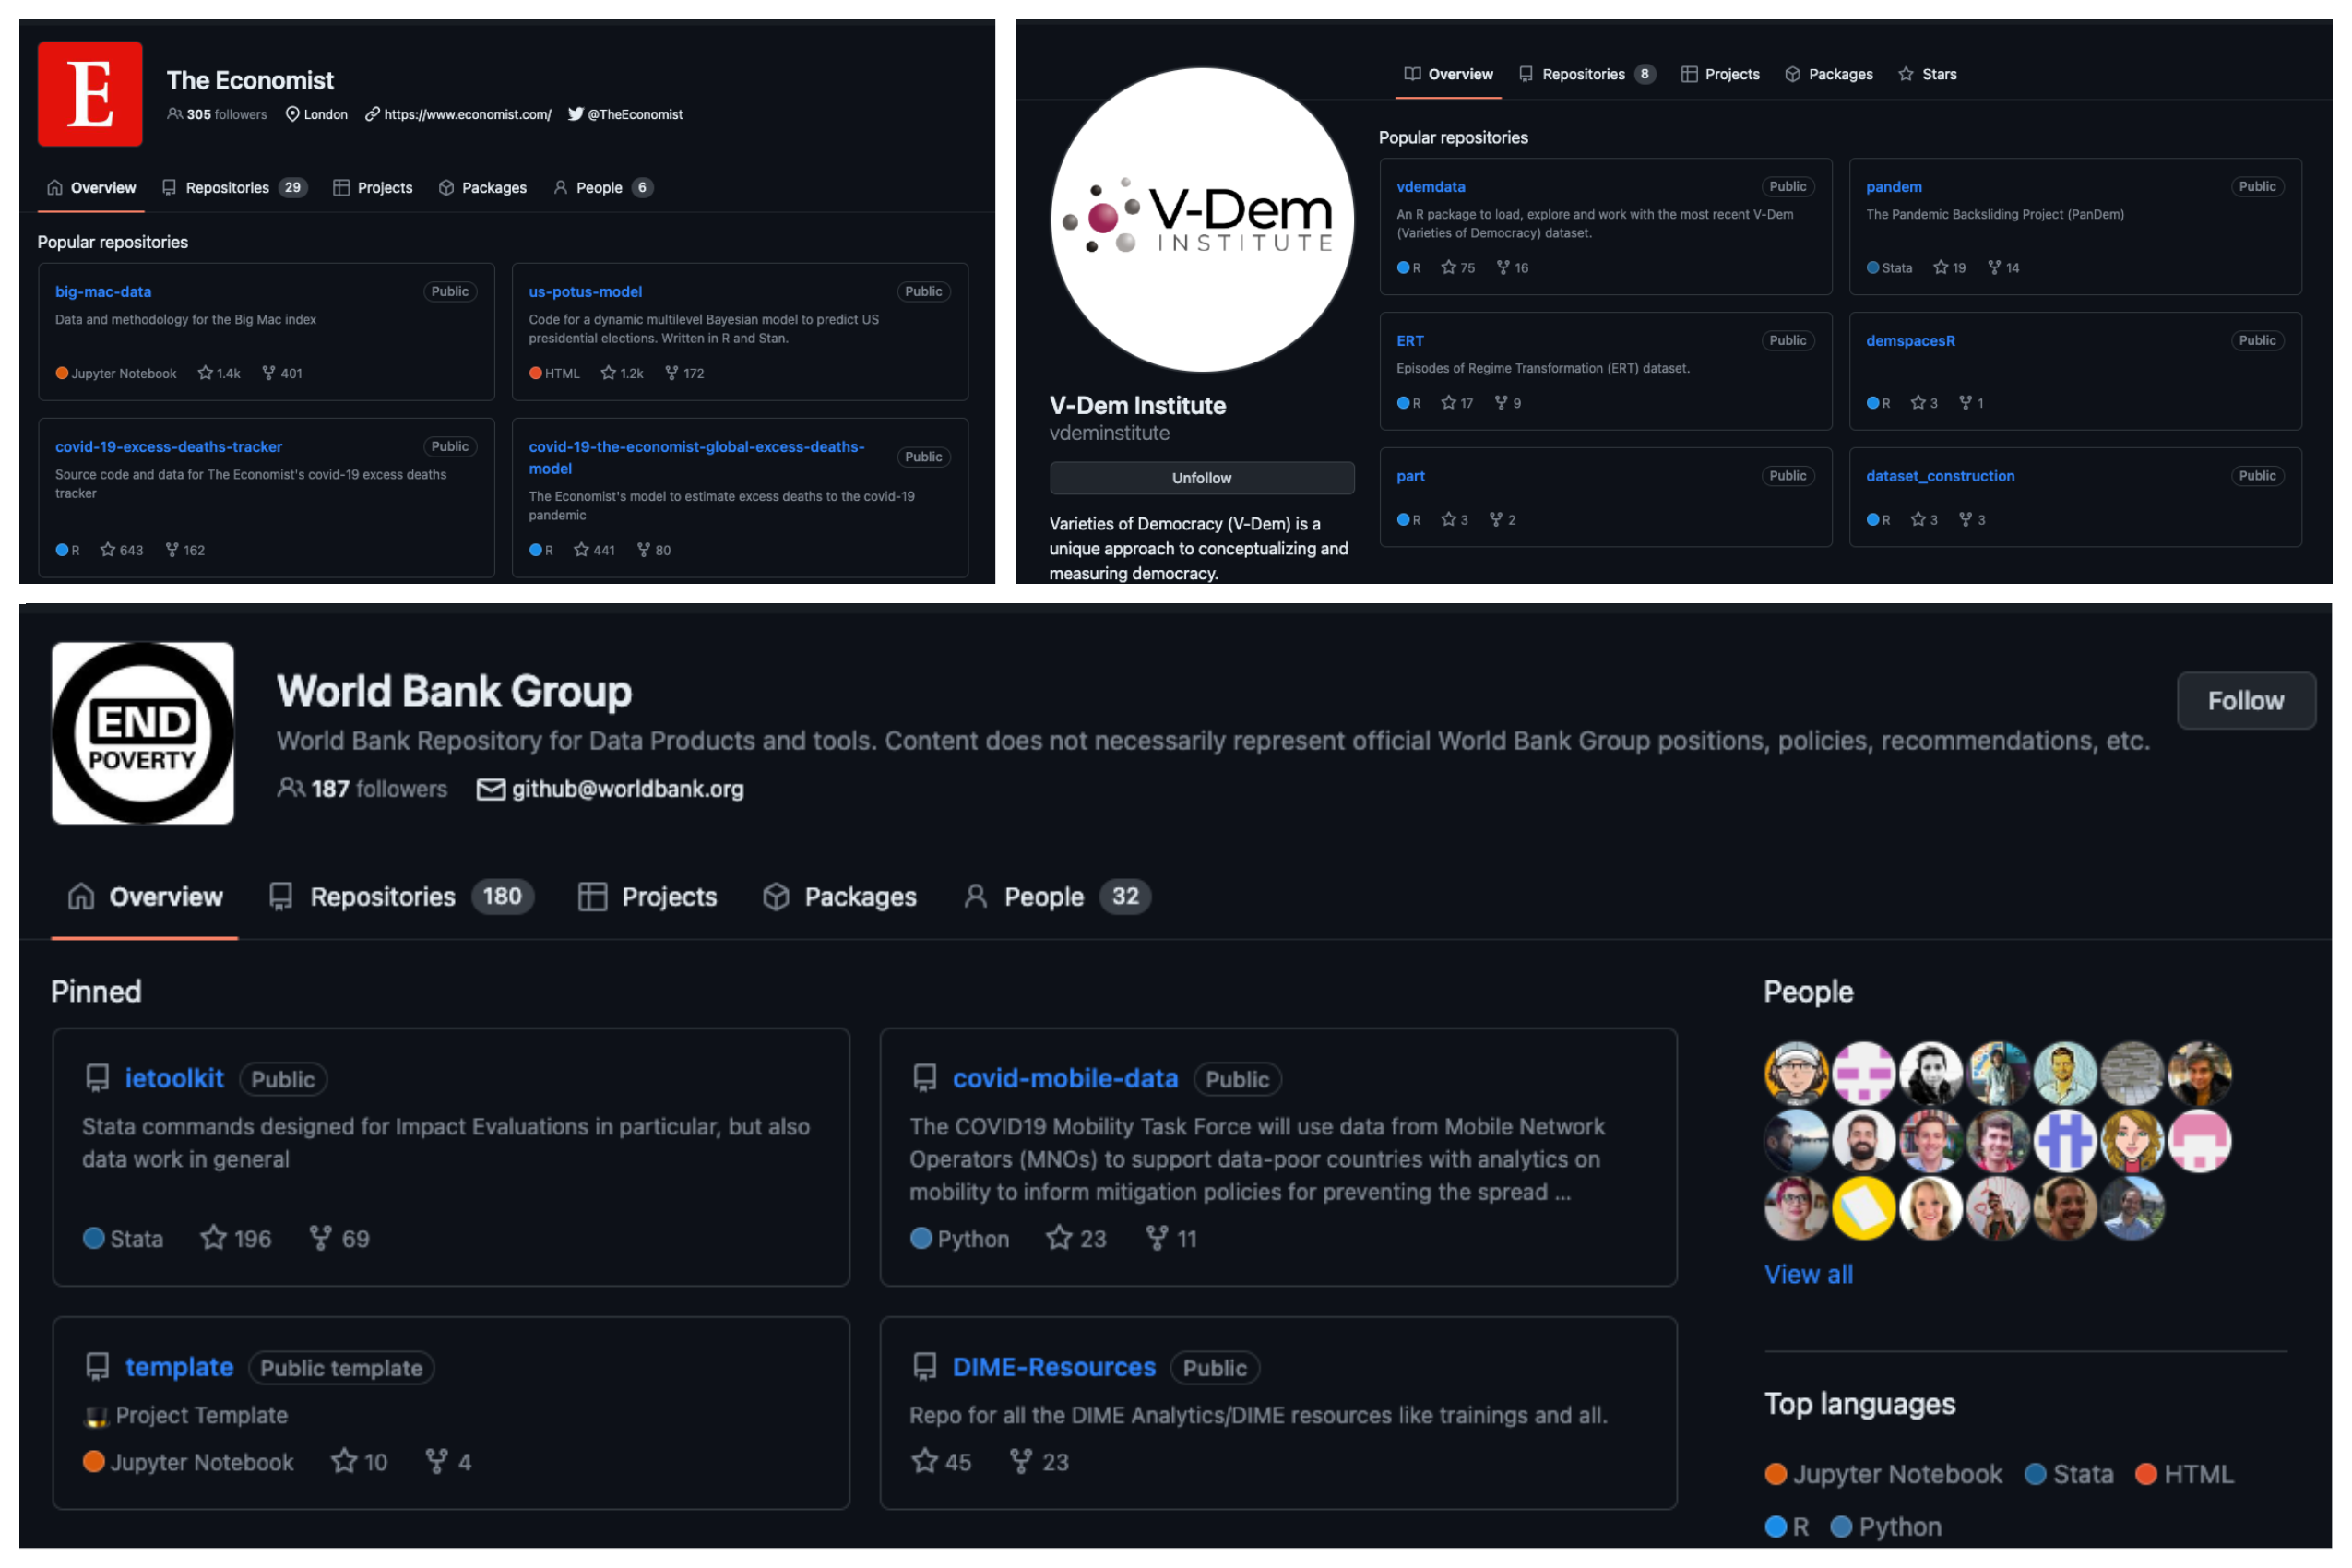
\includegraphics{media/github-ex.png}
\end{frame}

\begin{frame}[fragile]{Workflow tools: standardizing computer relative
paths}
\protect\hypertarget{workflow-tools-standardizing-computer-relative-paths}{}
\begin{itemize}
\item
  We manage our code assuming it can be replicable for anyone. This
  entails the need to standardize and synchronize the paths on our
  computer to the project.

  \begin{itemize}
  \tightlist
  \item
    Rproject or a code which synchronize the root directory
  \end{itemize}
\end{itemize}

\begin{Shaded}
\begin{Highlighting}[]
\DocumentationTok{\#\# +++++++++++++++++++++++++++++++++++++++++++++++++++++++++++++++++++++++++++++}
\DocumentationTok{\#\#}
\DocumentationTok{\#\# 2.  SharePoint Path                                                      {-}{-}{-}{-}}
\DocumentationTok{\#\#}
\DocumentationTok{\#\# +++++++++++++++++++++++++++++++++++++++++++++++++++++++++++++++++++++++++++++}

\CommentTok{\# SharePoint path}
\ControlFlowTok{if}\NormalTok{ (}\FunctionTok{Sys.info}\NormalTok{()[}\StringTok{"user"}\NormalTok{] }\SpecialCharTok{==} \StringTok{"johnDoe"}\NormalTok{) \{}
\NormalTok{  path2SP }\OtherTok{\textless{}{-}} \StringTok{"/Users/johnDoe/OneDrive{-}WJP/Data Analytics/"}

\NormalTok{\} }\ControlFlowTok{else} \ControlFlowTok{if}\NormalTok{ (}\FunctionTok{Sys.info}\NormalTok{()[}\StringTok{"user"}\NormalTok{] }\SpecialCharTok{==} \StringTok{"anaPerez"}\NormalTok{) \{}
\NormalTok{  path2SP }\OtherTok{\textless{}{-}} \StringTok{"/CloudStorage/OneDrive{-}WJP/Data Analytics/"}
  
\NormalTok{\} }\ControlFlowTok{else} \ControlFlowTok{if}\NormalTok{ (}\FunctionTok{Sys.info}\NormalTok{()[}\StringTok{"user"}\NormalTok{] }\SpecialCharTok{==} \StringTok{"kumikoNagato"}\NormalTok{)\{}
\NormalTok{  path2SP }\OtherTok{\textless{}{-}} \StringTok{"/Users/kumikoNagato/Library/OneDrive{-}WJP/Data Analytics/"}
  
\NormalTok{\} }\ControlFlowTok{else}\NormalTok{\{}
\NormalTok{  path2SP }\OtherTok{\textless{}{-}} \StringTok{"PLEASE INSERT YOUR PERSONAL PATH TO THE SP DAU DIRECTORY"}
  
\NormalTok{\}}
\end{Highlighting}
\end{Shaded}
\end{frame}

\hypertarget{our-workflow}{%
\section{Our Workflow}\label{our-workflow}}

\begin{frame}{Data analytics workflow for visualizations}
\protect\hypertarget{data-analytics-workflow-for-visualizations}{}
\begin{itemize}
\tightlist
\item
  \href{https://github.com/ctoruno/LAC-Reports}{\textbf{LAC Reports
  Workflow}}
\item
  \href{https://github.com/ctoruno/WJP-Data-Viz}{\textbf{Visualization
  Repository}}
\end{itemize}

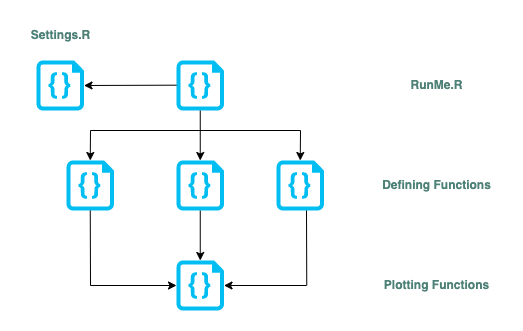
\includegraphics{media/code_structure.png}
\end{frame}

\begin{frame}[fragile]{Data analytics documentation}
\protect\hypertarget{data-analytics-documentation}{}
\begin{itemize}
\tightlist
\item
  \href{https://ctoruno.quarto.pub/wjp-r-handbook/coding.html}{\textbf{Handbook
  of DAU protocols}}
\item
  The documentation instills confidence in the estimations we are
  utilizing.
\item
  There are specific data-related decisions that we need to emphasize
  for the purpose of transparency.
\end{itemize}

\begin{Shaded}
\begin{Highlighting}[]
\NormalTok{  data\_subset.df }\OtherTok{\textless{}{-}}\NormalTok{ master\_data.df }\SpecialCharTok{\%\textgreater{}\%}
    \FunctionTok{filter}\NormalTok{(country }\SpecialCharTok{\%in\%}\NormalTok{ group) }\SpecialCharTok{\%\textgreater{}\%}
    
    \CommentTok{\# Latest year is different for Paraguay}
    \FunctionTok{mutate}\NormalTok{(}\AttributeTok{latestYear =} \FunctionTok{if\_else}\NormalTok{(country }\SpecialCharTok{==} \StringTok{"Paraguay"}\NormalTok{, }\DecValTok{2021}\NormalTok{, }\DecValTok{2022}\NormalTok{)) }\SpecialCharTok{\%\textgreater{}\%}
    \FunctionTok{mutate}\NormalTok{(}\AttributeTok{year =} \FunctionTok{if\_else}\NormalTok{(country }\SpecialCharTok{==} \StringTok{"Nicaragua"} \SpecialCharTok{\&}\NormalTok{ year }\SpecialCharTok{==} \DecValTok{2021}\NormalTok{, }\ConstantTok{NA\_real\_}\NormalTok{, year)) }\CommentTok{\# We didn\textquotesingle{}t use the data }
                                                                                  \CommentTok{\# from Nicaragua in 2021}
                                                                                  \CommentTok{\# index}
\end{Highlighting}
\end{Shaded}

\begin{itemize}
\item
  Good documentation facilitates the seamless integration of new team
  members and enables non-coding team members to comprehend the process
  effectively.
\item
  This is a good way to standardize the language of the project.
\end{itemize}
\end{frame}

\begin{frame}{Workflow prerequisites}
\protect\hypertarget{workflow-prerequisites}{}
\begin{itemize}
\item
  Outline made by Alex and the Data Analytics Team.
\item
  Design team specifications.
\item
  Data questionnaires and Data maps.
\item
  Data checks and analysis to take decisions.
\end{itemize}
\end{frame}

\hypertarget{challenges-and-questions-in-the-enpol-project}{%
\section{Challenges and questions in the ENPOL
project}\label{challenges-and-questions-in-the-enpol-project}}

\begin{frame}{Objective 1: General report}
\protect\hypertarget{objective-1-general-report}{}
\begin{itemize}
\item
  Objective 1: Summarize and present national and state-level criminal
  justice practices, trends, and deficiencies through use of ENPOL and
  other data sources.
\item
  This report is similar to the LAC reports; we can implement a similar
  workflow.
\item
  Nevertheless ¿How are we going to organize the previous analysis of
  the data? ¿What are the needs of the research team in the
  pre-analysis?
\item
  On which platform are we going to work?
\item
  Should this data repository be external to the main files?
\end{itemize}
\end{frame}

\begin{frame}{Objetive 2: Explanation and qualititative and quantitative
research report.}
\protect\hypertarget{objetive-2-explanation-and-qualititative-and-quantitative-research-report.}{}
\begin{itemize}
\item
  Objective 2: Prioritize and explain CJ system deficiencies revealed in
  Objective 1 through qualitative and quantitative research in 3-5
  states.
\item
  How can we organize a workflow that adds the qualitative and
  quantitative data?
\item
  Should this be managed in an inter-depend way?
\item
  What are the outputs that we are thinking in this report?
\end{itemize}
\end{frame}

\begin{frame}{Objetive 3: State government proposals for specific
criminal justice reform policies.}
\protect\hypertarget{objetive-3-state-government-proposals-for-specific-criminal-justice-reform-policies.}{}
\begin{itemize}
\item
  Beyond the production of key figures to support each proposal, is any
  additional visualization or analysis needed?

  \begin{itemize}
  \tightlist
  \item
    At this point, should we divide the workflow organization per
    product?
  \end{itemize}
\end{itemize}
\end{frame}

\hypertarget{conclusions}{%
\section{Conclusions}\label{conclusions}}

\begin{frame}{Conclusions}
\protect\hypertarget{conclusions-1}{}
\begin{itemize}
\item
  Thinking in a workflow before start all the production process allow
  us to save time and avoid repetitive process.
\item
  A workflow can help to replicate and update the work that we made.
\item
  A well-structured workflow facilitates easy comprehension of the
  process for all team members, enabling seamless integration for new
  members.
\item
  A workflow and a good documentation is a sign of good practice and
  rigor.
\item
  We can incorporate certain aspects of the data analytics workflow into
  the project. However, this project extends beyond mere report
  visualization. This presents us with an opportunity to expand the
  workflow, allowing us to replicate it in research and policy brief
  reports.
\end{itemize}
\end{frame}

\hypertarget{gracias}{%
\section{Gracias!}\label{gracias}}



\end{document}
